\begin{pastexam}[label={px:ccu-109-csb-03}]{中正資工所乙組 109 學年度 第 6 題}
（問答）

(20\%) Consider the following graph. Please write down the sequences of edges selected by the
following two algorithms, respectively.
\begin{enumerate}[label=(\alph*)]
\item (10\%) Kruskal's algorithm.
\item (10\%) Prim's algorithm (start from vertex a).
\end{enumerate}

\begin{center}
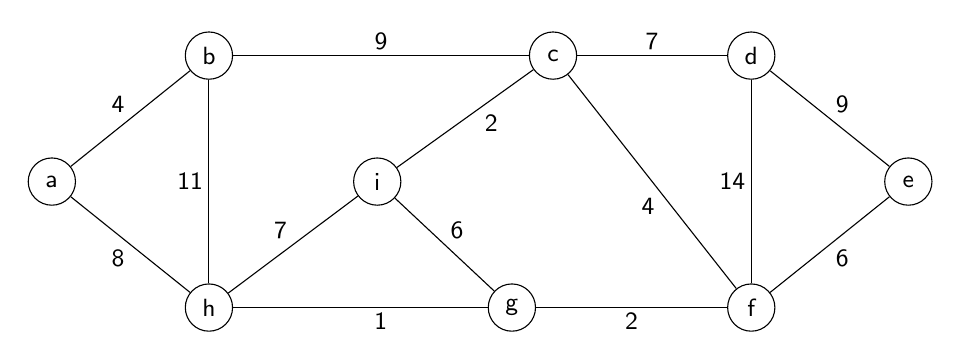
\begin{tikzpicture}[v/.style={circle,draw,minimum size=6mm,inner sep=0pt,font=\small\sffamily},
  w/.style={font=\small\sffamily,inner sep=2pt},x=0.95cm]
\node[v] (a) at (0,0) {a};
\node[v] (b) at (2.1,1.6) {b};
\node[v] (h) at (2.1,-1.6) {h};
\node[v] (i) at (4.35,0) {i};
\node[v] (c) at (6.7,1.6) {c};
\node[v] (g) at (6.15,-1.6) {g};
\node[v] (d) at (9.35,1.6) {d};
\node[v] (f) at (9.35,-1.6) {f};
\node[v] (e) at (11.45,0) {e};
\draw (a)--node[w,above left]{4}(b);
\draw (a)--node[w,below left]{8}(h);
\draw (b)--node[w,left]{11}(h);
\draw (b)--node[w,above]{9}(c);
\draw (c)--node[w,above]{7}(d);
\draw (c)--node[w,below right,pos=0.4]{2}(i);
\draw (c)--node[w,below left,pos=0.55]{4}(f);
\draw (d)--node[w,above right]{9}(e);
\draw (d)--node[w,left]{14}(f);
\draw (e)--node[w,below right]{6}(f);
\draw (h)--node[w,above left]{7}(i);
\draw (i)--node[w,above right]{6}(g);
\draw (h)--node[w,below,pos=0.58]{1}(g);
\draw (g)--node[w,below]{2}(f);
\end{tikzpicture}
\end{center}
\end{pastexam}

\begin{pastsoln}
圖有 $9$ 個頂點、$14$ 條邊，生成樹有 $8$ 條邊。 有幾組權重相同的邊（$2$、$4$、$6$、$7$、$9$
各有兩條），Kruskal 處理同權重的邊時先後順序可以任意，下面照表中的順序；最後會說明不管怎麼排，
選到的邊都一樣。

\textbf{(a)} 十四條邊依權重由小到大處理，兩端已經連通（在同一個集合）就略過，否則選進來並合併
兩個集合（資結書第~24.2~節）：
\begin{center}
\small
\begin{tabular}{rcrll}
\toprule
步 & 邊 & 權重 & 結果 & 選完後含這條邊的集合 \\
\midrule
1 & h--g & 1 & 選 & $\{g, h\}$ \\
2 & c--i & 2 & 選 & $\{c, i\}$ \\
3 & g--f & 2 & 選 & $\{f, g, h\}$ \\
4 & a--b & 4 & 選 & $\{a, b\}$ \\
5 & c--f & 4 & 選 & $\{c, f, g, h, i\}$ \\
6 & e--f & 6 & 選 & $\{c, e, f, g, h, i\}$ \\
7 & i--g & 6 & 略過：i--c--f--g 已連通 & \\
8 & c--d & 7 & 選 & $\{c, d, e, f, g, h, i\}$ \\
9 & h--i & 7 & 略過：h--g--f--c--i 已連通 & \\
10 & a--h & 8 & 選，已滿 $8$ 條 & $\{a, b, c, d, e, f, g, h, i\}$ \\
\bottomrule
\end{tabular}
\end{center}
剩下的 b--c（$9$）、d--e（$9$）、b--h（$11$）、d--f（$14$）兩端都已連通，不必再看。 Kruskal 選邊的
順序是
\[
(h, g),\ (c, i),\ (g, f),\ (a, b),\ (c, f),\ (e, f),\ (c, d),\ (a, h),
\]
總權重 $1 + 2 + 2 + 4 + 4 + 6 + 7 + 8 = 34$。 同權重的 (c, i) 和 (g, f)、(a, b) 和 (c, f)
先後對調也可以。 權重 $6$ 的兩條：如果先處理 i--g，那時 i 和 g 已經經過 c--f 連通（權重 $4$ 的
邊都處理完了），一樣略過，接著選 e--f；權重 $7$ 的 h--i 不論先後都會被略過。 所以選到的八條邊
不受同權重順序影響，這張圖的最小生成樹只有一棵。

\textbf{(b)} 從 a 開始執行 Prim 演算法，每回合取出 $\mathit{key}$ 最小、還不在樹裡的頂點，再用它的
邊更新鄰居（資結書第~24.3~節）。 格子寫 $\mathit{key}/\pi$，空白表示已在樹裡：
\begin{center}
\small
\setlength{\tabcolsep}{4pt}
\begin{tabular}{ccc*{9}{c}}
\toprule
回合 & 取出 & 加入的邊 & a & b & c & d & e & f & g & h & i \\
\midrule
1 & a & — & $0$ & $4/a$ & $\infty$ & $\infty$ & $\infty$ & $\infty$ & $\infty$ & $8/a$ & $\infty$ \\
2 & b & a--b & & $4/a$ & $9/b$ & $\infty$ & $\infty$ & $\infty$ & $\infty$ & $8/a$ & $\infty$ \\
3 & h & a--h & & & $9/b$ & $\infty$ & $\infty$ & $\infty$ & $1/h$ & $8/a$ & $7/h$ \\
4 & g & h--g & & & $9/b$ & $\infty$ & $\infty$ & $2/g$ & $1/h$ & & $6/g$ \\
5 & f & g--f & & & $4/f$ & $14/f$ & $6/f$ & $2/g$ & & & $6/g$ \\
6 & c & f--c & & & $4/f$ & $7/c$ & $6/f$ & & & & $2/c$ \\
7 & i & c--i & & & & $7/c$ & $6/f$ & & & & $2/c$ \\
8 & e & f--e & & & & $7/c$ & $6/f$ & & & & \\
9 & d & c--d & & & & $7/c$ & & & & & \\
\bottomrule
\end{tabular}
\end{center}
（每一列是取出那個頂點、更新完鄰居之後的值；取出的頂點那一格是它被取出時的值。） 幾個要注意的
更新：第 2 回合 b--h 是 $11$，不比 $\mathit{key}[h] = 8$ 小，不更新；第 4 回合 g--i 是 $6$，比
h--i 的 $7$ 小，$\mathit{key}[i]$ 改成 $6/g$；第 5 回合 f--c 是 $4$，把 c 從 $9/b$ 改成 $4/f$；
第 6 回合 c--i 是 $2$，再把 i 改成 $2/c$；第 8 回合 e--d 是 $9$，不比 $7$ 小。 每一回合要取的
最小值都只有一個，沒有平手。 Prim 選邊的順序是
\[
(a, b),\ (a, h),\ (h, g),\ (g, f),\ (f, c),\ (c, i),\ (f, e),\ (c, d),
\]
和 (a) 是同一組八條邊，總權重 $34$。
\end{pastsoln}
